
% This LaTeX was auto-generated from an M-file by MATLAB.
% To make changes, update the M-file and republish this document.

\documentclass{article}
\usepackage{graphicx}
\usepackage{color}

\sloppy
\definecolor{lightgray}{gray}{0.5}
\setlength{\parindent}{0pt}

\begin{document}



\subsection*{Contents - Largest $n$ such that we didn't run out of memory}

\begin{itemize}
\setlength{\itemsep}{-1ex}
   \item Jacobi
   \item BLKJacobi
   \item GS
   \item SOR
   \item GMRES
   \item PGMRES
   \item Plotting commands
\end{itemize}

        \color{lightgray} \begin{verbatim}
    =====================================================
      Solving the Convection-Diffusion equation with
         beta = -0.0097, gamma = -0.0195 and n = 512
    =====================================================

      Time using backslash = 1.9885
      solution norm = 6.3614e-06


\end{verbatim} \color{black}


\subsection*{Jacobi}
      \color{lightgray} \begin{verbatim}                      ------------------
                      |     Jacobi     |
                      ------------------
      Residual after error 2000 interations = 6.6688e-02
      Time to run Jacobi = 13.1997

\end{verbatim} \color{black}


\subsection*{BLKJacobi}
        \color{lightgray} \begin{verbatim}                      ------------------
                      |   BLK Jacobi   |
                      ------------------
      Residual after error 2000 interations = 6.3282e-02
      Time to run Jacobi = 28.6637

\end{verbatim} \color{black}


\subsection*{GS}

        \color{lightgray} \begin{verbatim}                      ------------------
                      |  Gauss-Siedel  |
                      ------------------
      Residual after error 2000 interations = 6.3550e-02
      Time to run GS = 19.1120

\end{verbatim} \color{black}


        \color{lightgray} \begin{verbatim}                      ------------------
                      |      SOR       |
                      ------------------

      Omega = 1.9
      Residual after error 2000 interations = 1.4998e-02
      Time to run SOR = 20.8581

\end{verbatim} \color{black}


       \color{lightgray} \begin{verbatim}                      -----------------
                      |     GMRES     |
                      -----------------
      Residual error after 1368 interations = 7.2598e-08
      Time to run CG = 4438.9891

\end{verbatim} \color{black}


\subsection*{PGMRES}

        \color{lightgray} \begin{verbatim}                      -----------------
                      |    PGMRES     |
                      -----------------
      Residual error after  417 interations = 1.2454e-07
      Time to run CG = 447.9855

\end{verbatim} \color{black}



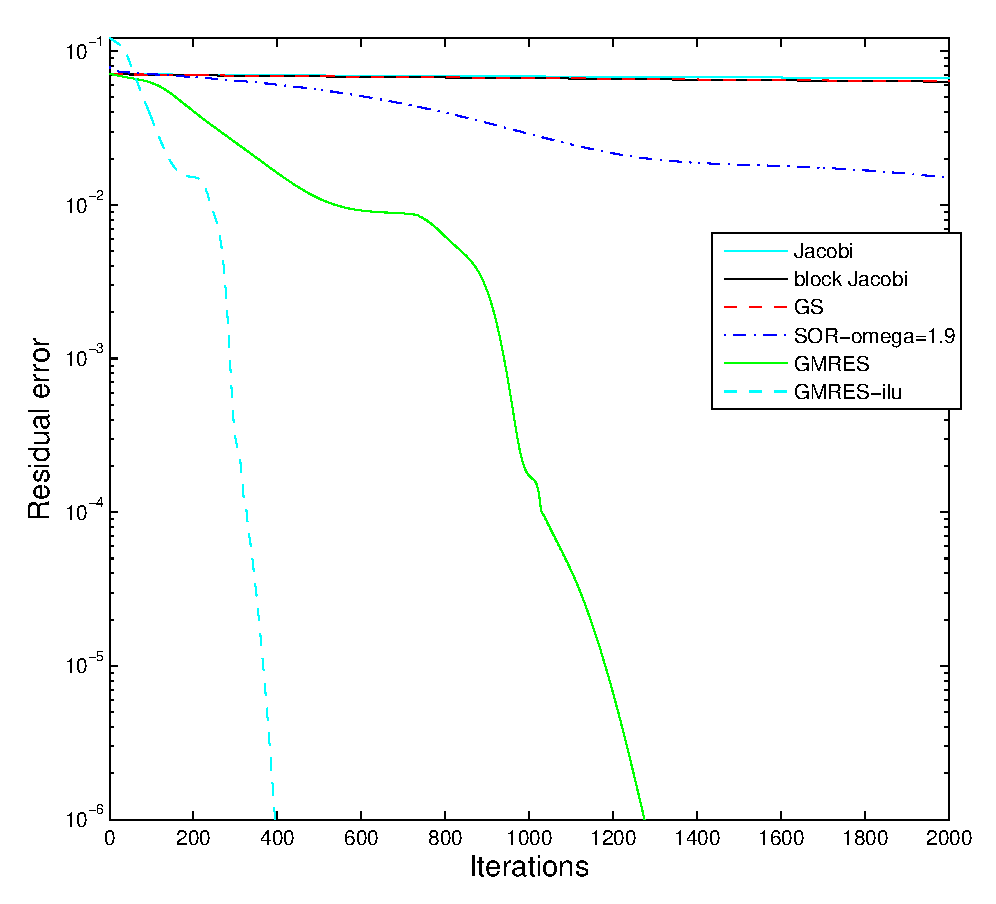
\includegraphics [width=3.75in]{A1q3_01.eps}


\end{document}

